\chapter{基于编码的密钥生成改进方案}
基于编码的加密方案,后续的改进工作主要集中在缩小公钥尺寸,提升解码效率两大方面。BBCRS公钥密码体制在安全性提升的同时,其Niederreiter版本保证了公钥尺寸与原始Niederreiter等同;在安全等级相同的情况下,加解密效率高于基于传统数论的RSA。为了缩小公钥尺寸,相关学者对各种能应用到McEliece加密方案的码进行了大量研究,比如低密度奇偶校验码,但是经过密码分析者的分析工作,这些码应用到McEliece加密方案中是不安全的,特别是改进的信息集解码攻击极易对这么设计产生威胁。但是BBCRS公钥密码体制的公钥设计,在一定程度上可以对码作出妥协,比如可以选择结构更紧凑的GRS码,在安全性上依然与应用Goppa的McEliece加密方案基本等同。

BBCRS公钥密码体制,在公钥的设计上是敢于突破的,不管是McEliece及其变体方案,还是Niederreiter及其变体方案,在公钥的设计上总是类似的,公钥与私钥之间总是保留着置换的相等关系。BBCRS选择直接将置换矩阵替换为其它形式的矩阵,在基于编码的公钥构造上提供了一些思路。本章内容,就是根据这种思路,提供了另一种公钥构造方式,该种方式可以达到BBCRS公钥密码体制中描述的公钥与私钥之间不再是置换相等的关系,从而在安全性上表现突出,在加解密表现上避免了BBCRS公钥密码体制出现的情况,是一种可取的改进方式。

\section{研究动机}
Marco Baldi等人在BBCRS公钥密码体制发表后,总结到方案采用GRS码既可以保证安全性的提升,又能带来公钥尺寸的减小。在同一种安全性级别,在加解密的操作复杂度显著低于RSA公钥密码体制。但是在2015年,有密码分析学者提出的密钥恢复攻击\cite{Couvreur2015A}可以在多项式时间内攻破采用GRS码的BBCRS公钥密码体制。具体来说,密码分析学者提出的攻击方案是针对矩阵$T$平均行重或列重范围在$[1,2]$的情况,利用矩阵$T$行列重量分布的特点,将BBCRS公钥密码体制的安全性降低到利用区分者攻击手法可恢复私钥的安全性。

如此以来,在BBCRS公钥密码体制的基础上,规避暴露出来的弱点,就是待解决的主要问题。首先就是关于码的选择,BBCRS公钥密码体制推荐使用GRS码,以便更好的利用GRS码结构紧凑的特性。但是这也成为后续攻击手段的切入点,虽然有掩藏结构的防范方法\cite{Berger2005How},但是在之后的密码分析中发现已不能满足安全性的要求。如果继而采用原始的Goppa码,就必须提升方案的信息利用率,不然在纠错能力$(\lfloor \frac{t}{m} \rfloor)$已经有所减少的情况下,对通信效率将是较大的影响。其次,方案在解密过程中,不仅要考虑中间结果超过码的最大纠错能力,还要考虑消除$\mathbf{e}R \neq \mathbf{0}$带来的穷举搜索的重复操作。另外,在加密过程中,随机选取的差错向量,重量已经有所减少,而且要满足$(\mathbf{a}_1 + \mathbf{a}_2 + ··· + \mathbf{a}_w) \cdot \mathbf{e}^\mathtt{T} = \mathbf{0}.$,这也带来了威胁较大的子码漏洞问题,虽然BBCRS公钥密码体制提出了解决之道,但是如果能放开这样的限制条件,或者改为其它的限制,方案的设计会更合理。

BBCRS公钥密码体制替换原始McEliece加密方案的置换矩阵,不仅消除了公钥与私钥之间置换相等的关系,而且矩阵$Q$的组成让我们有更多的细粒度的参数设定,比如$w$的值决定集合中矩阵的个数,$z$的值决定矩阵$R$的秩,BBCRS公钥密码体制Niederreiter版本要存储的公钥尺寸,和矩阵$R$的秩是息息相关的。这样的设计可以让我们根据不同的码的特点,空间效率等因素选择最优的参数来实现加解密。本文在设计基于BBCRS的改进方案时,也是将置换矩阵替换成多个矩阵计算结果的形式。BBCRS公钥密码体制在差错向量上的类似于陷门设定,在后续解密简化了步骤,这些都为新方案提供了思想指导。

\section{改进方向}
考虑到设计的可行性,本文主要对McEliece版本的BBCRS公钥密码体制进行公钥构造形式上的改进,参考以往McEliece方案的变体,随机非奇异矩阵$S$的作用基本不变,混淆生成矩阵为随机的矩阵,所以在新方案中,我们也保留这一左乘的形式。公钥的构造关键,就是原始McEliece方案的置换矩阵$P$这一部分,明文编码成含有错误码字,在进一步混淆私钥结构的过程中,就要考虑码字错误位数的扩散问题,置换矩阵因为每行每列都只有一个非零位,所以在计算$\mathbf{e}P^{-1}$的时候不会出现错误位数大于$\mathbf{e}$的汉明重量,即仍然可以正确的进行译码。回顾BBCRS公钥密码体制在这部分的考虑,其一是对差错向量有一定的约束,其二是对矩阵$T$在平均行重和列重做了规定,而且分析了解码失败的概率。于是在新公钥构造方式中,如何使约束成本最小化,混淆作用最大化就成了关键。

在BBCRS公钥密码体制的改进方向上,基本上确定矩阵$Q$是安全性和效率的关键部分,如何设计一个陷门,能把在加密过程中加入的混淆作用,在解密的时候消除掉是重中之重。首先我们想到可逆矩阵,可逆矩阵无疑是隐藏私钥矩阵的利器,但是我们不能忽略一个可逆矩阵与差错向量的计算结果,也就是说,如果采用可逆矩阵差错向量对汉明重量的要求,即码的纠错能力将毫无意义,因为可逆矩阵的扩散作用非常难以控制。

接下来,虽然可逆矩阵无法直接应用到公钥构造设计中,但是我们可以间接的加入可逆矩阵,也就是可逆矩阵作为参与者,承担一部分的作用。于是,关于替换置换矩阵的部分,就要像BBCRS那样,分为若干个部分。BBCRS中公钥密码体制中,采用的是一个秩固定的密集型矩阵和一个稀疏的广义置换矩阵,通过矩阵相加计算矩阵$Q$,在新公钥构造设计中,设想使一个特殊矩阵和可逆矩阵相加,来替换原始McEliece加密方案的置换矩阵。经过反复的推导,发现特殊矩阵与可逆矩阵相加这种方式,在解码的时候,无论特殊矩阵怎么努力,都无法吸收可逆矩阵在差错向量$\mathbf{e}$的扩散作用。但是,在反复推导中,我们逐渐认识到可逆矩阵不仅可以隐藏私钥结构,也可以隐藏差错向量,或者说任意与之做乘法的向量或矩阵。那么我们是不是可以包装一下可逆矩阵,让其暴露出来一个乘法结果,该乘法结果与差错向量$\mathbf{e}$满足一定的等式关系,从而在解密的时候可以利用这个等式关系,来达到控制差错向量错误位数的目的。

在改进方向上,我们反复斟酌,最终觉得这是可行的实现方法,下一节重点讨论方案的实现。

\section{方案设计}
在我们讨论的过程中,可逆矩阵基本确定要作为公钥构造设计的一部分,而另外一个特殊矩阵还需详细的分析。在公钥矩阵存储上,低秩矩阵的参与往往可以节约存储空间,但是在安全性上也有所下降,平衡好方案中各因素也是方案可行的关键。首先,本文改进的核心就是密钥生成算法,简要流程图见\ref{fig:keygenmethod_pdf}:

\begin{figure}[H]
	\centering
	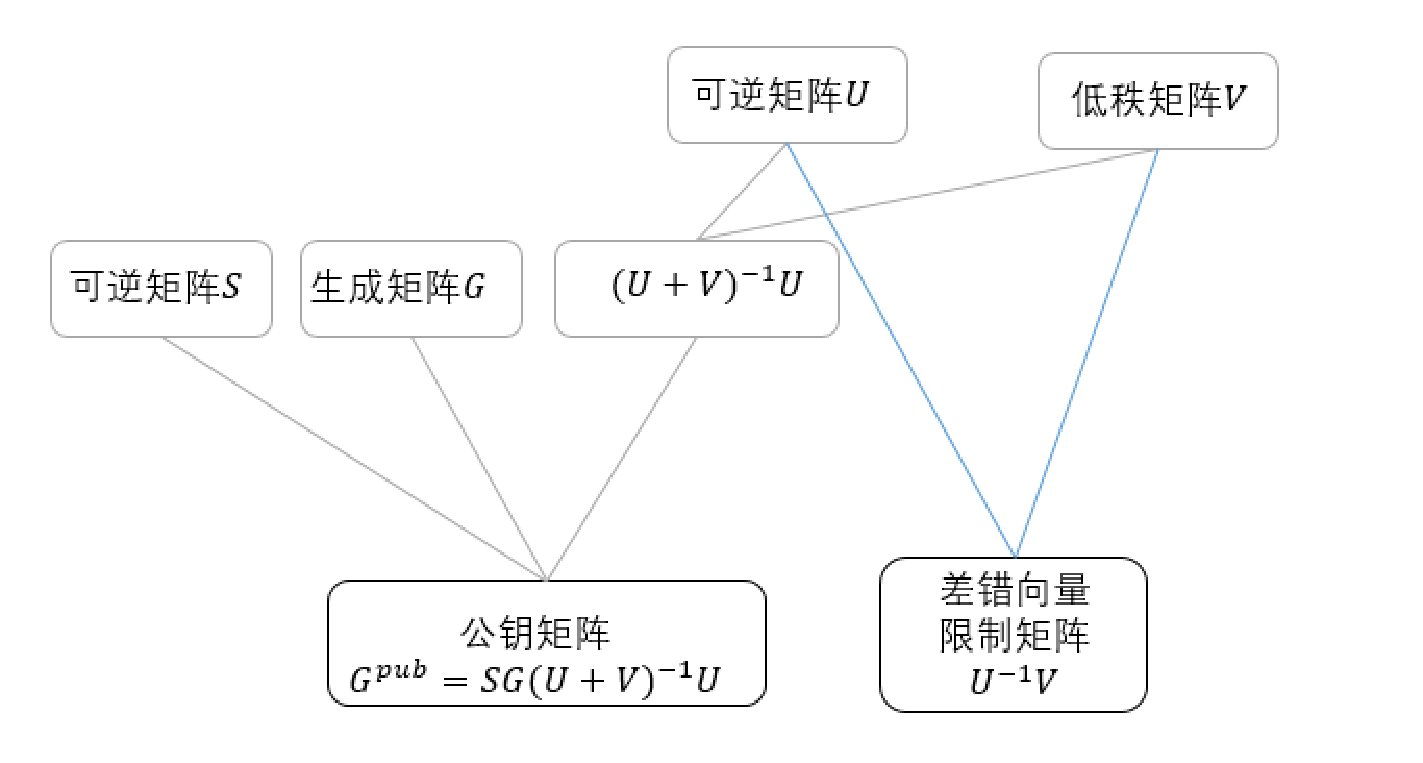
\includegraphics[width=15 cm]{fig/keygenmethod.pdf}
	\caption{密钥生成方式} %\vspace*{-1.0cm}
	\label{fig:keygenmethod_pdf}
\end{figure}

改进的密钥生成方式并不复杂,所以不会带来操作上的问题。观察公钥的设计可知,可逆矩阵$U$,与低秩矩阵$V$相加,使得满足可逆,外侧再右乘可逆矩阵$U$,结果必然是一个可逆矩阵。于是我们就达到了以可逆矩阵替换原始McEliece加密方案的置换矩阵,相比较于BBCRS公钥密码体制的$R+T$,一个可逆矩阵显然比其混淆性强,与此同时想要进行密钥恢复攻击几乎是不可能的。完整的密码加解密算法如下:
\begin{breakablealgorithm}
	\small
	\renewcommand{\algorithmicrequire}{\textbf{Input:}}
	\renewcommand{\algorithmicensure}{\textbf{Output:}}
	\caption{密钥生成改进方案}
	\label{alg:NewKeyGen}
	\begin{algorithmic}[1]
		\Require
		系统安全参数:$n,t \in N$,其中$t \ll n$。
		\Ensure
		公钥$(G^{pub},U^{-1}V)$,私钥$(S,D_\mathcal{C},U,V)$。
		\State
		密钥生成:对于给定的参数$n$和$t$,产生下列矩阵。
		\begin{itemize}
			\item 矩阵$G$:在有限域$\mathbb{F}$上的信息位数为$k$,最小距离为$d \geq 2t + 1$的Goppa码$\mathcal{C}$的$k \times n$阶生成矩阵。
			\item 矩阵$S$:$k \times k$阶的二元随机非奇异矩阵。
			\item 矩阵$U$:$n \times n$阶的二元随机可逆矩阵。
			\item 矩阵$V$:$n \times n$阶的二元随机低秩矩阵,秩为$r$。
		\end{itemize}
		\State
		然后计算方案的公钥$G^{pub} = S^{-1}G(U + V)^{-1}U$;接着计算另一公钥矩阵$U^{-1}V$。
		\begin{itemize}
			\item 公钥:$(G^{pub},U^{-1}V,t)$。
			\item 私钥:$(S,D_\mathcal{C},U,V)$,有效译码算法$D_\mathcal{C}$就是所用纠错码方案的陷门。
		\end{itemize}
	\end{algorithmic}
\end{breakablealgorithm}

在接下来的加解密算法中,我们同BBCRS一样,需要对差错向量做一些预备限制。

\begin{breakablealgorithm}
	\small
	\renewcommand{\algorithmicrequire}{\textbf{Input:}}
	\renewcommand{\algorithmicensure}{\textbf{Output:}}
	\caption{密钥生成改进方案加密算法}
	\label{alg:NeweEn}
	\begin{algorithmic}[1]
		\Require
		公钥$(G^{pub},U^{-1}V,t)$,长度为$k$的明文$\mathbf{m}$。
		\Ensure
		密文$\mathbf{c}$。
		\State
		随机选择一个汉明重量为$t$的随机向量$\mathbf{e} \in \mathbb{F}^n$,但是要满足:
		\begin{equation}
			wt(\mathbf{e})\leq t\quad \mbox{and}\quad \mathbf{e}\cdot U^{-1}V = \mathbf{0}.
		\end{equation}
		\State
		加密,产生密文:
		
		\centering $\mathbf{c} = \mathbf{m}G^{pub} + \mathbf{e}.$
	\end{algorithmic}
\end{breakablealgorithm}

为了确保解密过程含有错误的码字能被正确纠错,也就是码字含有错误的个数不能超过码的纠错能力,本方案对差错向量$\mathbf{e}$做了式 4.1的要求。式 4.1本质上式规定了差错向量$\mathbf{e}$的选择空间,之所以要求矩阵$V$是低秩矩阵,是因为低秩矩阵可以保证$U^{-1}V$的解空间足够大,足以保证差错向量$\mathbf{e}$的随机性,避免暴力攻击。

本方案的解密算法具体的实现如下:

\begin{breakablealgorithm}
	\small
	\renewcommand{\algorithmicrequire}{\textbf{Input:}}
	\renewcommand{\algorithmicensure}{\textbf{Output:}}
	\caption{密钥生成改进方案解密算法}
	\label{alg:NewDe}
	\begin{algorithmic}[1]
		\Require
		密文$\mathbf{c}$,私钥$(S,D_\mathcal{C},U,V)$。
		\Ensure
		明文$\mathbf{m}$。
		\State
		解密密文$\mathbf{c}$之前,首先利用私钥矩阵$U$计算:
		\begin{center}
			$\textbf{c}\cdot U^{-1} = \textbf{m}S^{-1}G(U+V)^{-1} \oplus\textbf{e}\cdot U^{-1}.$
		\end{center}
		\State
		接着利用私钥矩阵$U$与$V$的和$(U + V)$右乘上述结果:
		\begin{equation}
			\begin{aligned}
				\textbf{c}\cdot U^{-1}(U+V) &= \textbf{m}S^{-1}G \oplus\textbf{e}\cdot U^{-1}(U+V) \\
				& = \textbf{m}S^{-1}G \oplus  \textbf{e} \oplus \textbf{e}\cdot U^{-1}V \\
				& = \textbf{m}S^{-1}G \oplus  \textbf{e}.
			\end{aligned}
		\end{equation}
		
		\State
		观察上一步的结果,对其进行译码,因为上一步的计算结果可以看成为是码的一个含有$t$个错误的码字,而且码字含有的错误必然不会超过码的纠错能力,所以经过译码可以得到:
		\begin{center}
			$\mathbf{m}S^{-1}G = D_\mathcal{C}(\textbf{c}\cdot U^{-1}(U+V)).$
		\end{center}
		
		\State
		最后,令集合$J \subseteq \{0,1,2,...,n\}$,需要通过矩阵变换使$G_j^{pub}$可逆,则进行如下计算可以得到明文。
		\begin{center}
			$\mathbf{m} = (\mathbf{m}S^{-1}G)_j(G_j)^{-1}S.$
		\end{center}		
	\end{algorithmic}
\end{breakablealgorithm}

综上,加密的计算方式同原始的McEliece加密方案,明文通过编码并加入一些错误处理成合理的码字,解密过程同样要利用到编码的纠检错机制,消除加入的差错向量的影响,才能进而正确进行解密操作。在加密过程中,我们同样对差错向量$\mathbf{e}$作出了一定的约束,但是BBCRS公钥密码体制因此而导致的子码漏洞问题在本方案中是不存在的。我们保证差错向量的选择空间足够大,而且使其纠错能力上升到码的实际纠错能力,而BBCRS公钥密码体制在纠错能力上是有所折扣的。

解密工作类似于加密中混淆作用的反过程,但是要注意的是,加密过程中,差错向量是直接追加上去的,并没有参与混淆计算,也就是差错向量的重量和影响一直是差错向量本身带来的影响,而解密过程就大不相同,因为解密过程中,差错向量要跟解密时用到的私钥矩阵相计算,如此以来,一定要找到控制差错向量错误位数的方法,不然解密工作就会走向失败。由式 4.2我们可以得出结论,本方案是可以正确进行加解密的基于编码的密码方案。

从方案的设计我们可以看到,原始的McEliece加密方案的置换矩阵,细化这部分的构造,将有很多的改进空间。如BBCRS公钥密码体制在广义置换矩阵$T$的基础上,再加上了一个密集矩阵$R$,而矩阵$R$实际上是两个元素都是随机矩阵的集合通过计算而得。这两个矩阵集合的元素,就成为公钥构造的关键因素这也为本方案更细粒度的控制可逆矩阵和低秩矩阵提供了进一步的努力方向,此外,也提供了对于差错向量的控制的指导思路。

\section{安全性分析}
自原始McEliece加密方案在1978年提出以来,针对其进行的密码分析工作和相关变形方案一直在研究之中。基于编码的公钥加密方案需要满足最基本的安全等级就是被动攻击下的单向安全性,毫无疑问,BBCRS公钥密码体制以及本文的改进方案都可以达到这样的要求。但是在接近实际的应用中,这样的安全等级是不可靠的,我们必须满足更好的安全要求,比如自适应选择密文攻击下的不可区分性。BBCRS在文中已经讨论了要达到自适应选择密文攻击下的不可区分性这种安全级别的方案实现,对安全级别起重要作用的就是替换原McEliece加密方案置换矩阵的矩阵$Q$所含有的私钥部分,而本文提出的是更为有效的可逆矩阵$(U + V) ^ {-1}U$来代替置换矩阵。其次,差错向量的约束,以及后续的解密工作对比BBCRS公钥密码体制和本文方案,本文都有安全性和解密效率的提升。接下来我们从常见的对基于编码的加密方案的攻击来阐述本文方案的安全性。

\subsection{解码攻击}
经典的解码攻击是在不需要了解任何码的结构信息情况下,对一个随机线性码进行正确解码。也就是说,敌手不需要知道任何私钥信息,但是可以从密文$\mathbf{c}$中恢复明文$\mathbf{m}$。首先我们先解释一下传统的伴随式译码攻击。

\begin{enumerate}
	\item 敌手获得公钥矩阵$G^{pub}$,然后根据$G^{pub} \cdot (H^{pub})^\mathtt{T} = \mathbf{0}$计算出公开的校验矩阵$H^{pub}$;
	\item 接下来对密文$\mathbf{c}$计算其伴随式,过程如下:
	\begin{equation}
		\begin{aligned}
			\mathbf{c}(H^{pub})^\mathrm{T} & = (\mathbf{m}G^{pub} \oplus\mathbf{e})(H^{pub})^\mathtt{T} \\
			& = \mathbf{m}G^{pub}(H^{pub})^\mathtt{T} + \mathbf{e}(H^{pub})^\mathtt{T} \\
			& = \mathbf{e}(H^{pub})^\mathtt{T}.
		\end{aligned}
	\end{equation}
	\item 通过式 4.3的验证,敌手会努力寻找正确的差错向量$\mathbf{e}$,于是就可以从$\mathbf{c} = \mathbf{m}G^{pub} + \mathbf{e}$式中提取$\mathbf{m}G^{pub}$,通过高斯消除法就可以进一步获取明文$\mathbf{m}$。		
\end{enumerate}

在这个过程中,敌手需要产生所有重量不超过码的纠错能力$t$的差错向量$\mathbf{e}$,就是采用暴力破解法,在敌手尝试攻击我们的系统时,需要尝试验证的工作量可以通过如下计算得到:

\begin{equation}\label{Eq:numberOfErrorVectionInOriginalAttack}
\sum_{i=1}^{t} \dbinom{n}{i}
\end{equation}

前文已经提到,BBCRS公钥密码体制的纠错能力已经不再是码的纠错能力$t$,而是$wt(\mathbf{e}) \leq \lfloor t/2m \rfloor$,于是BBCRS公钥密码体制在抵御经典解码攻击时的工作量是:

\begin{equation}\label{Eq:numberOfErrorVectionInBBCRSScheme}
\sum_{i=1}^{\frac{t}{2m}} \dbinom{n}{i}
\end{equation}

在这里$n$指得是码字的长度,一般情况下,只要$n,t$是正常的参数级别,要想从式 4.4来暴力破解几乎式不可能的,但是对于BBCRS公钥密码体制,式 4.5显示暴力搜索的空间已经减小很多,而且解码攻击已经加入了很多新的技术来加速攻击的效果。我们的方案在实际执行的时候,差错向量$\mathbf{e}$的选择空间也不再是式 4.4所描述的完全空间,而是受式 4.1的约束和私钥矩阵$V$的秩$r$的影响,暴力搜索差错向量$\mathbf{e}$需要尝试$2^{n-r}$次,在McEliece公钥加密方案推荐的参数下,这将是非常大的数字,所以说在这一点我们改进的方案会更安全。

仅仅在经典的伴随式译码攻击下保证安全性是远远不够的,在基于编码的加密算法的解码攻击中,最常见,也是发展最迅速的就是信息集解码攻击。其主要思想是通过确定$k$个坐标位置,使得生成矩阵对应的$k$列构成满秩矩阵,并且接收到的码字对应的位置都是没有错误的,由此获得传递中的明文信息。对于确定这样$k$个坐标位置的算法很多,比如Stern算法,MMT算法等。但是无论如何,信息集解码攻击都是依赖差错向量非错误位的个数,也就是零位的个数,这样才能使$k$的选取成功概率更大。相较于BBCRS公钥密码体制,我们扩展了加密方案差错向量的最大错误位数,对于信息集解码攻击意味着更高的复杂度,从而保证了改进方案的安全性。

一些论文中,提出了加速解码攻击的方案,可以快速的找到正确的差错向量$\mathbf{e}$,以恢复明文信息。其基本的思路是将差错向量$\mathbf{e}$分成若干个部分,将汉明重量分配到每一部分中,根据各部分汉明重量总和跟差错向量本身的汉明重量相等,从而提高暴力搜索差错向量$\mathbf{e}$的速度。相关学者已经指出,该种解码攻击手段极易在$q$元域上攻击失败,我们的改进方案是很容易应用到$q$元域上的。不仅如此,我们可以适当的减小码的长度,以使$t/n$的比值增大,如此以来,信息集攻击想要在没有错误的坐标位置还原明文信息将变得更加困难,所以说我们的方案是可以抵御各类解码攻击威胁的。

\subsection{密钥恢复攻击}
密钥恢复攻击,意味着敌手已经获得了加解密设计的密钥信息,敌手可以自由加密或解密信息,也就是密码系统被完全攻破。大部分情况下,这是很难做到的,而且敌手的野心一般也不需要这么大,敌手有时候只想获得特定的密文信息,而不是耗费大量攻击成本去还原密钥。关于BBCRS公钥密码体制在密钥恢复攻击的攻击情况,相关学者在\cite{Couvreur2015A}中就提出可以在多项式时间内攻破采用GRS码的BBCRS公钥密码体制,该篇文章的主要工作主要使BBCRS公钥密码体制的安全性下降,其中的私钥矩阵$T$退化成一个普通的置换矩阵,然后根据已经研究出的攻击手段进行后续攻击。该种攻击针对的情况是很特殊的,其对BBCRS公钥密码体制中的参数$m$要求是在$[1, 2]$范围内。BBCRS公钥密码体制就可以通过调整采用的码来抵御这种攻击,或者对$m$的值进行一定程度的优化。同样,我们的新方案也可以直接规避开GRS码,其实也可以保留GRS码,接下来我们重点讨论一下改进方案在密钥恢复攻击的下的安全层次。

对BBCRS公钥密码体制多项式时间内的密钥恢复攻击,目的是为了恢复私钥矩阵$R$,$T$。具体来说,首先敌手会通过算法定位私钥矩阵$T$的行重或者列重大于$1$的位置;然后通过线性变换将其转换为置换矩阵,接下来的攻击工作会利用GRS码的结构性质及其平方码的构造。对我们的改进方案来说,我们的私钥$(S,D_\mathcal{C},U,V)$不含有置换矩阵的成分,非奇异矩阵$U$和低秩矩阵$V$对密钥恢复攻击的工作是一项极大的挑战,特别需要关注的是$(U+V)^{-1}U$的部分,这是一个非奇异矩阵,将使得密钥恢复攻击无处着手,密钥恢复攻击很多时候会用到区分者攻击的手段,下一小节我们详细讨论区分者的攻击情况。

在这里我们讨论相关学者提出的一个对McEliece加密方案变体进行高效密钥恢复攻击的方法。该方案变体采用的是附带卷积码信息的Goppa码,作者指出,对私钥附带的信息带有很大的随机性,所以其密钥结构已经不在矩阵敌手可以利用的代数结构,私钥的隐藏效果显著,于是就可以采用代数结构较强的码。但是这并不完全有效,在作者的分析中,可以利用公钥寻找一些汉明重量较低的码字,用其还原附带的卷积码结构。实际上,这种高效的密钥恢复攻击对我们的方案也是无效的。上述不安全的方案的私钥生成矩阵经过置换矩阵$P$的作用,紧接着穿插进卷积部分的列,置换矩阵$P$经由我们的私钥矩阵$(U+V)^{-1}U$替换,将会杜绝这种风险。还有一种针对准循环码的密钥恢复攻击,也是利用了置换矩阵参与公钥构造的特点,对于我们的方案公钥的构造方式,此种攻击则不会构成威胁。

\subsection{区分者攻击}
正如我们上文提到的,区分随机线性码与Goppa码是$NP$困难问题,但是当我们使用结构特殊或者结构性较强的码时,就有可能遭受区分者攻击,区分者攻击技术在基于编码的加密方案的密码分析中用得很多,目的是为了获取我们的私钥结构信息。抵御区分者攻击的关键就是对私钥进行有效的混淆,在我们的改进方案中,对公钥的构造使得公钥看起来更随机,在其它方案中,置换矩阵的存在总是敌手利用相关技术获得信息的入口,消除置换矩阵的混淆作用时敌手进行攻击的前提。而本文的新方案采用右乘一个可逆矩阵$(U+V)^{-1}U$的做法,这是很有效的,解决根源威胁的方式,我们接下来还是要讨论几种不同的区分者攻击方式,大部分都是针对GRS码的分析,我们也推荐采用除GRS码以外的码。但是为了公钥尺寸的问题,我们也可以调整参数,使得采用GRS码同样保证是安全的。

我们的新方案,推荐采用码率较高的码,以适应码长对公钥尺寸的影响。无独有偶,在文章中,作者提出了一种多项式时间内针对高码率的区分者攻击。事实上,该文章攻击的思想是利用与码息息相关的多项式在线性系统中的解空间问题,期间涉及到密钥恢复的一些手法,最后可以由推导的公式判断码的种类。作者提供了通用随机码,替换代码和Goppa代码的显式公式。可以发现这项工作与私有代码的生成矩阵结构密切相关,并且该攻击方法不可避免的利用了McEliece加密方案的置换矩阵$P$,在不包含置换矩阵的新公钥密码体制下,这将是无效的,我们还可以根据攻击情况调整码的种类选择。调整参数也是我们的预防手段之一。

假设我们采用GRS代码,即便我们能够安全地隐藏其结构,我们也必须考虑为它设计的区分攻击。 GRS代码的平方具有异常小的维度,在使用GRS代码的一些密码系统中,可以通过计算公钥的平方码的维度来检测公钥的生成矩阵中的随机列信息。在某些情况下,计算各种子码以及公钥的各种穿插版本的平方码维度仍然可以从公钥中获取私钥的一部分信息。 它们的共同弱点是密钥生成中的置换操作。 不失一般性的情况下,我们的计划在这方面是具有明显的安全优势。

\section{效率分析}
在本节我们讨论新方案在存储效率和计算效率两方面的表现,为了清晰说明新方案的改进效果,我们会结合经典的McEliece变体方案及BBCRS公钥密码体制的效率分析。我们会利用具体的公式估计改进方案在操作复杂度上的表现。

相比较经典McEliece加密方案,BBCRS公钥密码体制及本文的改进方案都在密钥生成阶段,解密阶段多出一些操作,但是,这些操作都是简单的位运算,而且改进方案是稳定,有序的进行计算的,在这一点上,BBCRS公钥密码体制会有意外情况需要处理。由上文可知,解码过程有可能解码失败,而且在处理差错向量$\mathbf{e}$的约束问题时,需要进行穷举操作,对译码的效率非常不利。而在我们的改进方案中,是不需要考虑这些操作的。在密钥生成阶段,我们较经典方案多出一次可逆矩阵的乘法计算,另外我们还计算了$U^{-1}V$,为了对差错向量进行约束使其合法合理的被正确纠错。其实在产生私钥矩阵很$U,V$之后,上述两个计算可以并行执行,并不会影响正确的结果。

与此同时我们需要额外的$n \times n$的存储空间,也就是存储$U^{-1}V$。在存储方面较BBCRS公钥密码体制显示出了劣势。这对于推广基于编码的加密方案非常不利,因为公钥的尺寸问题正是阻碍方案的发展主要因素之一。 幸运的是,我们可以进行其他调整以避免公钥尺寸的膨胀。 矩阵$U^{-1}V$的存储大小可以减小到$n \times n - r \times r$。因为奇异矩阵可以转换为仅包含单位矩阵的部分。我们的改进方案还原了原始McEliece加密方案的纠错能力,这意味着每个码字都可以携带更多的信息位,这也使得我们能够适当地减少明文消息的长度,同时也保证通信的信息效率要求。实际上,当我们需要获得一个满足条件$\mathbf{e}U^{-1}V = \mathbf{0}$的随机差错向量$\mathbf{e}$时,我们只是从齐次线性方程的解空间中随机选取一个解。所以说解空间的大小至关重要,我们必须保证差错向量的足够随机化以预防暴力破解。

关于解密过程,我们首先计算$\mathbf{c}U^{-1}$,然后我们进行矩阵乘法$\mathbf{c}U^{-1}(U + V)$。根据经典的安全参数,与McEliece公钥加密方案的变体相比,本方案需要额外$n$长度向量和$n \times n$矩阵之间的基本乘法。我们需要再次考虑适当的$n$值以加速我们的密码系统。接下来,解码工作将按顺序执行。让我们在这里回顾BBCRS公钥密码体制的解决方案,它是在矩阵乘法$\mathbf{c}Q$之后猜测满足$\mathbf{e}R = \lambda$的正确值$\lambda$。随着$z$值的变化,例如$z = 1$增加到$z = n$的过程中,猜测的操作次数将呈指数级增加。假设$q$为有限域$\mathbb{F}_q$中的元素数,每次选择一个可能值$\lambda$时,解密过程都将进行迭代计算,判断能否解码结果,直到解码操作成功为止。显然,迭代计算阶段涉及解码算法和其他操作,这极大地影响了密码体制的速度,接下来我们会统计实验数据来说明方案之间在各方面的差异。

\section{实验结论}
一方面,参数$n$从不同方面影响着我们提出的新方案,例如公钥的大小,解密的效率等。为了系统可用性,我们做了一些推导实验,以确保从整个公钥密码系统的表现选择合适的参数$n$。 另一方面,参数$r$,即矩阵$V$的秩依然是必不可少的影响成分。上文提到,差错向量的选取空间和随机化效果取决于$r$的值。本推导实验假设采用Goppa码作为私钥,参数的设置如:$q = 2, \mathbb{F}_{2^{10}}, N_c$,$N_c$表示Goppa解码的操作复杂次数,我们可以采用如下的计算方式:

\begin{equation}
	N_c=n+4(\log_2^2n)t^2+2(\log_2^2n)t+(\log_2^2n)(2t+1)+\frac{(n-k)^2}{2}.
\end{equation}

我们可以在表 \ref{bbcrsScheme}和表 \ref{ourScheme}看到详细的对比。

\begin{table}[h]
	\begin{center}
		\caption{BBCRS Scheme ($m=1.5,z=1$)}\label{bbcrsScheme}
		\begin{tabular}{ccccc}
			\hline
			$t$ & $n$& $k$ & public key size& decryption operations\\
			\hline
			13& 390& 195& 76050& 1.5$N_c$\\
			19& 570& 285& 162450& 1.5$N_c$\\
			27& 910& 405& 368550& 1.5$N_c$\\
			34& 1020& 510& 520200& 1.5$N_c$\\
			\hline
		\end{tabular}
	\end{center}
\end{table}

\begin{table}[h]
	\begin{center}
		\caption{Our Improved Scheme}\label{ourScheme}
		\begin{tabular}{ccccc}
			\hline
			$t$ & $n$& $k$ & public key size& decryption operations\\
			\hline
			13& 260& 130& 84500& $N_c$\\
			19& 380& 190& 180500& $N_c$\\
			27& 540& 270& 364500& $N_c$\\
			34& 680& 340& 578000& $N_c$\\
			\hline
		\end{tabular}
	\end{center}
\end{table}

\section{本章小结}
本章详细介绍了新的基于编码的加密方案,从研究动机,改进方向,方案实现等方面阐述了方案的由来,在改进的过程中,理论依据和总结经验扮演着十分重要的角色。实际在后面方案的实现上,出现过一些偏差,主要还是构造公钥的时候考虑不够全面,随机的差错向量在方案中的位置不够清晰。差错向量是加密这随机选取的一个满足约束的向量,加密者本身无法提前知道,所以解密的时候要利用译码算法纠正错误,而敌手则会通过解码攻击争取获得正确的差错向量从而获取密钥信息。

本章后半部分介绍了在相关攻击下新方案的安全性,方案的效率分析以及实验结论。我们在错误向量空间和公钥大小之间做了一些妥协。从安全性的角度来看,我们通过调整$k$来保证抵御攻击的能力。从公钥大小的角度来看,由于具有纠错能力参数$t$的上限还原,我们适当减少了消息的长度,并保持了密码的安全性。对于我们描述的已知攻击,我们已经改进了基本的构造因素,因此攻击者没有有效的方法可以切入,从而我们的方案更可靠。我们的方案中也可以采用多种码,因为我们会很好地隐藏密钥的结构。